
\de{ĐỀ THI HỌC KỲ I NĂM HỌC 2022-2023}{THPT Chuyên Hạ Long - Quảng Ninh}
\begin{center}
	\textbf{PHẦN 1 - TRẮC NGHIỆM}
\end{center}
\Opensolutionfile{ans}[ans/ans]
\begin{ex}%[0D1B1-5]%[Dự án đề kiểm tra HK1-BCTuan]%[THPT Chuyên Hạ Long Quảng Ninh]
	Tìm mệnh đề {\bf sai.}
	\choice
	{$\exists x\in\mathbb{R}, x^2+5x+6=0$}
	{$\exists x\in\mathbb{R},x<3x$}
	{$\forall x\in\mathbb{R},x^2+2x+3>0$}
	{\True $\forall x\in\mathbb{R}, x^2\ge x$}
	\loigiai{
		Khi $x=\dfrac{1}{2}$ thì $\dfrac{1}{4}\ge \dfrac{1}{2}$ là sai, do đó mệnh đề \lq\lq$\forall x\in\mathbb{R}, x^2\ge x$\rq\rq\ là mệnh đề sai.
	}
\end{ex}
\begin{ex}%[0D1B3-2]%[Dự án đề kiểm tra HK1-BCTuan]%[THPT Chuyên Hạ Long Quảng Ninh]
	Tìm mệnh đề {\bf sai.}
	\choice
	{$(A\cap B)\subset B$, với mọi tập $A$, $B$}
	{\True $(A\cup B)\subset (A\cap B)$, với mọi tập $A$, $B$}
	{$A\subset (A\cup B)$, với mọi tập $A$, $B$}
	{$A\setminus B \subset A$, với mọi tập $A$, $B$}
	\loigiai{
		$(A\cup B)\subset (A\cap B)$, với mọi tập $A$, $B$ là mệnh đề sai.	
	}
\end{ex}
\begin{ex}%[0H1Y1-3]%[Dự án đề kiểm tra HK1-BCTuan]%[THPT Chuyên Hạ Long Quảng Ninh]
	Cho $0^\circ <\alpha <90^\circ$. Tìm mệnh đề đúng.
	\choice
	{$\tan (90^\circ-\alpha)=-\cot\alpha$}
	{$\cot (90^\circ-\alpha)=-\tan\alpha$}
	{\True $\cos (90^\circ-\alpha)=\sin\alpha$}
	{$\sin (90^\circ-\alpha)=-\cos\alpha$}
	\loigiai{
		Có $\cos (90^\circ-\alpha)=\sin\alpha$.	
	}
\end{ex}
\begin{ex}%[0D3B2-1]%[Dự án đề kiểm tra HK1-BCTuan]%[THPT Chuyên Hạ Long Quảng Ninh]
	Xác định parabol $(P)\colon y=2x^2+bx+c$, biết rằng $(P)$ có đỉnh $I(-1;-2)$.
	\choice
	{$y=2x^2-4x$}
	{$y=2x^2-3x+4$}
	{\True $y=2x^2+4x$}
	{$y=2x^2-4x+4$}
	\loigiai{
		Vì $I(-1;-2)$ là đỉnh parabol nên $\heva{&-\dfrac{b}{4}=-1\\&2-b+c=-2}\Leftrightarrow\heva{&b=4\\& c=0.} $\\
		Vậy $y=2x^2+4x$.
	}
\end{ex}
\begin{ex}%[0D4Y2-1]%[Dự án đề kiểm tra HK1-BCTuan]%[THPT Chuyên Hạ Long Quảng Ninh]
	Tam thức $f(x)=2x^2+2x+5$ nhận giá trị dương khi và chỉ khi
	\choice
	{$x\in (-2;+\infty)$}
	{\True $x\in\mathbb{R}$}
	{$x\in (-\infty;2)$}
	{$(0;+\infty)$}
	\loigiai{
		Ta có $\Delta'=1-2\cdot 5=-9<0$ và $a=2>0$ nên $f(x)>0 , \forall x\in\mathbb{R}$.	
	}
\end{ex}
\begin{ex}%[0H1B2-2]%[Dự án đề kiểm tra HK1-BCTuan]%[THPT Chuyên Hạ Long Quảng Ninh]
	Một tam giác có ba cạnh $13$, $14$, $15$ có diện tích bằng bao nhiêu?
	\choice
	{\True $84$}
	{$\sqrt{84}$}
	{$42$}
	{$\sqrt{168}$}
	\loigiai{
		Nửa chu vi là $p=21$.\\
		Diện tích là $S=\sqrt{21(21-13)(21-14)(21-15)}=84$.	
	}
\end{ex}
\begin{ex}%[0H1B2-1]%[Dự án đề kiểm tra HK1-BCTuan]%[THPT Chuyên Hạ Long Quảng Ninh]
	Cho tam giác $ABC$ có $AC=4$ cm, $\widehat{A}=60^\circ$, $\widehat{B}=45^\circ$. Tính $BC$.
	\choice
	{$\sqrt{6}$}
	{\True $2\sqrt{6}$}
	{$2+2\sqrt{3}$}
	{$2\sqrt{3}-2$}
	\loigiai{
		Ta có $\dfrac{BC}{\sin A}=\dfrac{AC}{\sin B}\Rightarrow BC=\dfrac{AC\cdot\sin A}{\sin B}=\dfrac{4\sin 60^\circ}{\sin 45^\circ}=2\sqrt{6}$.	
	}
\end{ex}
\begin{ex}%[0D3K2-3]%[Dự án đề kiểm tra HK1-BCTuan]%[THPT Chuyên Hạ Long Quảng Ninh]
	\immini{Cho hàm số $y=ax^2+bx+c$ có đồ thị như hình bên. Tìm mệnh đề đúng.
		\choice
		{$a<0,b<0,c<0$}
		{$a<0,b>0,c>0$}
		{\True $a<0,b<0,c>0$}
		{$a>0,b<0,c>0$}}{
		\begin{tikzpicture}[scale=1,font=\footnotesize,line join = round, line cap = round, >= stealth]
			\def\a{-3} \def\b{2} \def\c{-1} \def\d{3}
			\coordinate (O) at (0,0)node[above left]{$O$};
			\coordinate (M) at (2,3);
			\draw[->] (\a,0)--(\b,0)node[below]{$x$};
			\draw[->] (0,\c)--(0,\d)node[right]{$y$};
			\foreach \p/\g in {} \draw[fill] (\p) circle(.5pt)node [shift={(\g:.3)}] {$\p$};
			\draw (-2,-.5) parabola bend ((-.5,2)(1,-.5);
	\end{tikzpicture}}
	\loigiai{
		Từ đồ thị suy ra $a<0$, $c>0$.\\
		Hoành độ đỉnh $-\dfrac{b}{2a}<0\Rightarrow b<0$.\\
		Vậy $a<0$, $b<0$, $c>0$.
	}
\end{ex}
\begin{ex}%[0H2B3-5]%[Dự án đề kiểm tra HK1-BCTuan]%[THPT Chuyên Hạ Long Quảng Ninh]
	\immini{Cho tam giác $ABC$, gọi $M$ là trung điểm $AB$ và $N$ là một điểm trên cạnh $AC$ sao cho $NC=2NA$. Gọi $K$ là trung điểm của $MN$. Tìm mệnh đề đúng.
		\choice
		{$\overrightarrow{AK}=\dfrac{1}{6}\overrightarrow{AB}+\dfrac{1}{4}\overrightarrow{AC}$}
		{$\overrightarrow{AK}=\dfrac{1}{4}\overrightarrow{AB}-\dfrac{1}{6}\overrightarrow{AC}$}
		{\True $\overrightarrow{AK}=\dfrac{1}{4}\overrightarrow{AB}+\dfrac{1}{6}\overrightarrow{AC}$}
		{$\overrightarrow{AK}=\dfrac{1}{6}\overrightarrow{AB}-\dfrac{1}{4}\overrightarrow{AC}$}}{
		\begin{tikzpicture}[scale=1,font=\footnotesize,line join = round, line cap = round, >= stealth]
			\coordinate (B) at (0,0);
			\coordinate (C) at (4,0);
			\coordinate (A) at (65:5);
			\coordinate (M) at ($(A)!1/2!(B)$);
			\coordinate (N) at ($(A)!1/3!(C)$);
			\coordinate (K) at ($(M)!1/2!(N)$);
			\draw (A)--(B)--(C)--cycle;
			\draw (M)--(N) (A)--(K);
			\foreach \p/\g in {A/90,B/-90,C/-90,M/120, N/10, K/-80} \draw[fill] (\p) circle(.5pt) node [shift={(\g:.3)}] {$\p$};
	\end{tikzpicture}}
	\loigiai{
		Ta có $\overrightarrow{AK}=\dfrac{1}{2}\left(\overrightarrow{AM}+\overrightarrow{AN}\right)=\dfrac{1}{4}\overrightarrow{AB}+\dfrac{1}{6}\overrightarrow{AC}$.	
	}
\end{ex}
\begin{ex}%[0D3B2-5]%[Dự án đề kiểm tra HK1-BCTuan]%[THPT Chuyên Hạ Long Quảng Ninh]
	\immini{Một chiếc cổng hình parabol dạng $y=-\dfrac{1}{2}x^2$ có chiều rộng $d=8$ m. Điểm cao nhất của cổng cách mặt đất một khoảng bằng bao nhiêu mét?
		\choice
		{$16$}
		{\True $8$}
		{$4$}
		{$32$}}{\begin{tikzpicture}[scale=.4, font=\footnotesize, line join=round, line cap=round, >=stealth]
			\draw[->] (-4.5,0)--(0,0) node[above right]{$O$}--(4.5,0) node[below]{$x$};
			\draw[->] (0,-8.5) --(0,1.5) node[right]{$y$};
			\draw [domain=-4:4, samples=100] %
			plot (\x, {(-0.5)*(\x)^2});
			\draw[fill] (0,0) circle (1pt);
			\foreach \x/\g in {} 
			\draw[fill] (\x,0) circle(.5pt)node [shift={(\g:.3)}] {$\x$};
			\foreach \y/\g in {} 
			\draw[fill] (0,\y) circle(.5pt)node [shift={(\g:.3)}] {$\y$};
	\end{tikzpicture}}
	\loigiai{
		Khi $x=4\Rightarrow y=-8$. Suy ra chiều cao của cổng là $8$ m.	
	}
\end{ex}
\begin{ex}%[0D2B1-2]%[Dự án đề kiểm tra HK1-BCTuan]%[THPT Chuyên Hạ Long Quảng Ninh]
	\immini{Phần không bị gạch (không kể biên) ở hình bên là hình biểu diễn miền nghiệm của bất phương trình nào dưới đây?
		\choice
		{\True $x-y<0$}
		{$x+y<0$}
		{$x-y>0$}
		{$x+y>0$}}{
		\begin{tikzpicture}[scale=1, font=\footnotesize, line join=round, line cap=round, >=stealth]
			\draw[->] (-1.5,0)--(0,0) node[below right]{$O$}--(2,0) node[below]{$x$};
			\draw[->] (0,-2) --(0,2.5) node[right]{$y$};
			\draw [domain=-2:2, samples=100] %
			plot (\x, {(\x)});
			\draw[dashed] (1,0)--(1,1)--(0,1);
			\draw[fill] (0,0) circle (1pt);
			\foreach \x/\g in {1/-90} 
			\draw[fill] (\x,0) circle(.5pt)node [shift={(\g:.3)}] {$\x$};
			\foreach \y/\g in {1/180} 
			\draw[fill] (0,\y) circle(.5pt)node [shift={(\g:.3)}] {$\y$};
			\path[pattern = north west lines,opacity=0.3] (-2,-2)--(2,-2)--(2,2)--cycle;
	\end{tikzpicture}}
	\loigiai{
		Từ điểm $(1;1)$ thuộc đường thẳng biên và điểm $(0;1)$ thuộc miền nghiệm nên là hình biểu diễn cho bất phương trình $x-y<0$.	
	}
\end{ex}
\begin{ex}%[0D3Y1-4]%[Dự án đề kiểm tra HK1-BCTuan]%[THPT Chuyên Hạ Long Quảng Ninh]
	Điểm nào sau đây thuộc đồ thị hàm số $y=\dfrac{1}{x-1}$.
	\choice
	{$M(2;0)$}
	{$N(0;-2)$}
	{\True $P(2;1)$}
	{$Q(1;1)$}
	\loigiai{
		Khi $x=2\Rightarrow y=\dfrac{1}{2-1}=1$ nên điểm $P(2;1)$ thuộc đồ thị hàm số $y=\dfrac{1}{x-1}$.	
	}
\end{ex}
\begin{ex}%[0D3Y2-3]%[Dự án đề kiểm tra HK1-BCTuan]%[THPT Chuyên Hạ Long Quảng Ninh]
	Trục đối xứng của parabol $(P)\colon y=2x^2+6x+3$ là đường thẳng
	\choice
	{$y=-3$}
	{\True $x=-\dfrac{3}{2}$}
	{$y=-\dfrac{3}{2}$}
	{$x=-3$}
	\loigiai{
		Trục đối xứng là $x=-\dfrac{b}{a}=-\dfrac{3}{2}$.	
	}
\end{ex}
\begin{ex}%[0H1B3-2]%[Dự án đề kiểm tra HK1-BCTuan]%[THPT Chuyên Hạ Long Quảng Ninh]
	\immini{Hai chiếc tàu thuỷ cùng xuất phát từ một vị trí $A$, đi thẳng theo hai hướng tạo với nhau góc $60^\circ$. Tàu $B$ chạy với tốc độ $20$ hải lí một giờ. Tàu $C$ chạy với tốc độ $15$ hải lí một giờ. Sau hai giờ, hai tàu cách nhau bao nhiêu hải lí? Kết quả gần nhất với số nào sau đây?
		\choice
		{$21$ hải lí}
		{$18$ hải lí}
		{$61$ hải lí}
		{\True $36$ hải lí}}
	{
		\begin{tikzpicture}[line join=round, line cap=round,>=stealth,scale=1]
			\foreach \x in {1,2,3}
			\foreach \y in {0,1,2,3,4,5}
			\draw(0.25+\y,\x-0.25)--(\y,\x-0.25) ;
			\foreach \x in {1,2,3}
			\foreach \y in {0,1,2,3,4,5}
			\draw(-0.25+\y,\x-0.75)--(\y,\x-0.75) ;
			\tkzDefPoints{0/0/A,4/0/B,1.5/2.5/C}
			\tkzDefMidPoint(A,B) \tkzGetPoint{40}
			\tkzDefMidPoint(A,C) \tkzGetPoint{30} 
			\tkzDrawPoints[fill=black](A,B,C)
			\tkzDrawSegments(A,B A,C)
			\fill plot [smooth cycle] coordinates{(3.75,0)(4.25,0)(4.3,0.2)(4.15,0.2)(4.15,0.3)(4.05,0.3)(4.05,0.4)(3.95,0.4)(3.95,0.3)(3.85,0.3)(3.85,0.2)(3.7,0.2)} ;
			\fill plot [smooth cycle] coordinates{(1.25,2.5)(1.75,2.5)(1.8,2.7)(1.65,2.7)(1.65,2.8)(1.55,2.8)(1.55,2.9)(1.45,2.9)(1.45,2.8)(1.35,2.8)(1.35,2.7)(1.2,2.7)} ;
			\tkzLabelPoints[below](A,B,C,40)
			\tkzLabelPoints[left](30)
		\end{tikzpicture}
	}
	\loigiai{
		Sau $ 2$ giờ tàu $ B$ đi được $ 40$ hải lí, tàu $ C$ đi được $ 30$ hải lí. \\
		Vậy tam giác $ ABC$ có $ AB=40$, $AC=30$ và $ \widehat{A}=60^\circ$. \\
		Áp dụng định lí cô-sin vào tam giác $ ABC$, ta có
		$$ a^2=b^2+c^2-2bc\cdot\cos A=30^2+40^2-2\cdot 30\cdot 40\cdot \cos 60^\circ=1300\Rightarrow a\simeq 36.$$ 
		Vậy sau $ 2$ giờ, hai tàu cách nhau khoảng $ 36$ hải lí.}
\end{ex}
\begin{ex}%[0D2Y1-2]%[Dự án đề kiểm tra HK1-BCTuan]%[THPT Chuyên Hạ Long Quảng Ninh]
	Điểm $M(-2;1)$ thuộc miền nghiệm của bất phương trình nào sau đây?
	\choice
	{$x-2y>0$}
	{\True $4x-5y<0$}
	{$x+y>0$}
	{$x+3y<0$}
	\loigiai{
		Thay toạ độ điểm $M(-2;1)$ vào bất phương trình	$4x-5y<0$, ta được $-13<0$ là mệnh đề đúng.
	}
\end{ex}
\begin{ex}%[0D1B3-4]%[Dự án đề kiểm tra HK1-BCTuan]%[THPT Chuyên Hạ Long Quảng Ninh]
	Cho hai tập hợp $A=[1;3]$ và $B=[m;m+1]$. Tìm tất cả các giá trị của tham số $m$ để $B\subset A$.
	\choice
	{$m=2$}
	{$m=1$}
	{$1<m<2$}
	{\True $1\le m\le 2$}
	\loigiai{
		Ta có $B\subset A\Leftrightarrow \heva{&m\ge 1\\&m+1\le3}\Leftrightarrow 1\le m\le 2 $.	
	}
\end{ex}
\begin{ex}%[0D4B1-2]%[Dự án đề kiểm tra HK1-BCTuan]%[THPT Chuyên Hạ Long Quảng Ninh]
	Tam thức bậc hai $f(x)=-x^2+5x-6$ nhận giá trị dương khi và chỉ khi
	\choice
	{$x\in (2;+\infty)$}
	{\True $x\in (2;3)$}
	{$x\in (-\infty; 2)$}
	{$(3;+\infty)$}
	\loigiai{
		$f(x)=-x^2+5x-6>0\Leftrightarrow x\in(2;3)$. 	
	}
\end{ex}
\begin{ex}%[0H2B3-1]%[Dự án đề kiểm tra HK1-BCTuan]%[THPT Chuyên Hạ Long Quảng Ninh]
	Cho tam giác $OAB$ vuông cân tại $O$, cạnh $OA=a$. Tính $|2\overrightarrow{OA}-\overrightarrow{OB}|$.
	\choice
	{\True $a\sqrt{5}$}
	{$2a\sqrt{2}$}
	{$a$}
	{$(1+\sqrt{2})a$}
	\loigiai{\immini{Vẽ $\overrightarrow{OC}=2\overrightarrow{OA}$. Ta có\\
			$|2\overrightarrow{OA}-\overrightarrow{OB}|=|\overrightarrow{OC}-\overrightarrow{OB}|=|\overrightarrow{BC}|=BC$.\\
			Xét $\triangle OBC$ vuông tại $O$ có\\
			$BC=\sqrt{OB^2+OC^2}=a\sqrt{5}$.}{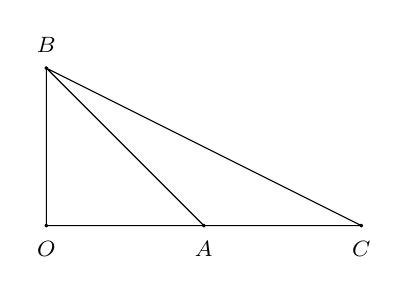
\begin{tikzpicture}[scale=1, font=\footnotesize, line join=round, line cap=round, >=stealth]
				\coordinate (O) at (0,0);
				\coordinate (A) at (2,0);
				\coordinate (B) at (0,2);
				\coordinate (C) at (4,0);
				\draw (A)--(B)--(O)--cycle
				(A)--(C)--(B)
				;
				\foreach \x/\g in {A/-90,B/90,O/-90,C/-90} \draw[fill] (\x) circle(.5pt)node [shift={(\g:.3)}] {$\x$};
		\end{tikzpicture}}	
	}
\end{ex}
\begin{ex}%[0D1B1-6]%[Dự án đề kiểm tra HK1-BCTuan]%[THPT Chuyên Hạ Long Quảng Ninh]]
	Tìm mệnh đề đúng.
	\choice
	{\True Điều kiện đủ để có ít nhất một trong hai số $a$, $b$ là số dương là $a+b>0$}
	{Điều kiện cần và đủ để một tứ giác là hình chữ nhật là nó có hai đường chéo bằng nhau}
	{Điều kiện cần và đủ để một số tự nhiên chia hết cho $15$ là số đó chia hết cho $5$}
	{Điều kiện cần để $a+b$ là một số hữu tỉ là $a$ và $b$ điều là số hữu tỉ}
	\loigiai{
		Điều kiện đủ để có ít nhất một trong hai số $a$, $b$ là số dương là $a+b>0$ là mệnh đề đúng.	
	}
\end{ex}
\begin{ex}%[0D3Y1-2]%[Dự án đề kiểm tra HK1-BCTuan]%[THPT Chuyên Hạ Long Quảng Ninh]
	Tìm tập xác định $\mathscr{D}$ của hàm số $y=\sqrt{6-3x}-\sqrt{x-1}$.
	\choice
	{$\mathscr{D}=[1;2]$}
	{\True $\mathscr{D}=[1;3]$}
	{$\mathscr{D}=[-1;2]$}
	{$\mathscr{D}=(1;2)$}
	\loigiai{
		Hàm số xác định khi $\heva{&6-3\ge 0\\&x-1\ge 0}\Leftrightarrow \heva{&x\le 3\\&x\ge 1}\Leftrightarrow 1\le x\le 3$.\\
		Vậy tập xác định $\mathscr{D}=[1;3]$.
	}
\end{ex}
\begin{ex}%[0D3B2-1]%[Dự án đề kiểm tra HK1-BCTuan]%[THPT Chuyên Hạ Long Quảng Ninh]
	Tìm parabol $(P)\colon y=ax^2+3x-2$, biết rằng parabol cắt trục $Ox$ tại điểm có hoành độ bằng $2$.
	\choice
	{\True $y=-x^2+3x-2$}
	{$y=-x^2+x-2$}
	{$y=-x^2+3x-3$}
	{$y=x^2+3x-2$}
	\loigiai{
		Vì parabol cắt trục $Ox$ tại điểm có hoành độ bằng $2$ nên suy ra $4a+6-2=0\Leftrightarrow a=-1$.\\
		Vậy $y=-x^2+3x-2$.	
	}
\end{ex}
\begin{ex}%[0D3B2-2]%[Dự án đề kiểm tra HK1-BCTuan]%[THPT Chuyên Hạ Long Quảng Ninh]
	Cho hàm số $y=-x^2+4x+1$. Khẳng định nào sau đây {\bf sai?} 
	\choice
	{Trên khoảng $(3;+\infty)$ hàm số nghịch biến}
	{Hàm số nghịch biến trên khoảng $(2;+\infty)$ và đồng biến trên khoảng $(-\infty;2)$}
	{\True Hàm số nghịch biến trên khoảng $(4;+\infty)$ và đồng biến trên khoảng $(-\infty;4)$}
	{Trên khoảng $(-\infty;-1)$ hàm số đồng biến}
	\loigiai{
		Hàm số $y=-x^2+4x+1$ đồng biến trên khoảng $(-\infty;2)$ và nghịch biến trên khoảng $(2;+\infty)$.
	}
\end{ex}
\begin{ex}%[0H2B2-2]%[Dự án đề kiểm tra HK1-BCTuan]%[THPT Chuyên Hạ Long Quảng Ninh]
	Cho hình bình hành $ABCD$ có $O$ là giao điểm của hai đường chéo. Tìm mệnh đề {\bf sai.}
	\choice
	{$|\overrightarrow{BA}+\overrightarrow{BC}|=|\overrightarrow{DA}+\overrightarrow{DC}|$}
	{\True $\overrightarrow{AB}+\overrightarrow{CD}=\overrightarrow{AB}+\overrightarrow{CB}$}
	{$\overrightarrow{OA}+\overrightarrow{OB}+\overrightarrow{OC}+\overrightarrow{OD}=\overrightarrow{0}$}
	{$\overrightarrow{AC}=\overrightarrow{AB}+\overrightarrow{AD}$}
	\loigiai{\immini{$\overrightarrow{AB}+\overrightarrow{CD}=\overrightarrow{AB}+\overrightarrow{CB}$ là mệnh đề sai.}{\begin{tikzpicture}[scale=1, font=\footnotesize, line join=round, line cap=round, >=stealth]
				\coordinate (A) at (0,0);
				\coordinate (B) at (3,0);
				\coordinate (C) at (30:5);
				\coordinate (D) at ($(A)+(C)-(B)$);
				\coordinate (O) at ($(A)!1/2!(C)$);
				\draw (A)--(B)--(C)--(D)--cycle
				(A)--(C) (B)--(D)
				;
				\foreach \x/\g in {A/-90,B/-90,O/-100,C/45,D/90} \draw[fill] (\x) circle(.5pt)node [shift={(\g:.3)}] {$\x$};
		\end{tikzpicture}}
		
	}
\end{ex}
\begin{ex}%[0D3B2-3]%[Dự án đề kiểm tra HK1-BCTuan]%[THPT Chuyên Hạ Long Quảng Ninh]
	Hàm số nào sau đây có đồ thị là parabol với đỉnh $I(-1;3)$?
	\choice
	{$y=2x^2+x+2$}
	{$y=2x^2-4x-3$}
	{$y=2x^2-2x-1$}
	{\True $y=2x^2+4x+5$}
	\loigiai{
		Hàm số $y=2x^2+4x+5$ có đồ thị là parabol với đỉnh $I(-1;3)$.
	}
\end{ex}
\begin{ex}%[0H1B2-1]%[Dự án đề kiểm tra HK1-BCTuan]%[THPT Chuyên Hạ Long Quảng Ninh]
	Cho tam giác $ABC$ có $AB=4$ cm, $BC=7$ cm, $AC=9$ cm. Tính $\cos A$.
	\choice
	{$\cos A=\dfrac{1}{2}$}
	{$\cos A=\dfrac{1}{3}$}
	{\True $\cos A=\dfrac{2}{3}$}
	{$\cos A=-\dfrac{2}{3}$}
	\loigiai{
		Ta có $\cos A=\dfrac{AB^2+AC^2-BC^2}{2AB\cdot AC}=\dfrac{16+81-49}{2\cdot 4\cdot 9}=\dfrac{2}{3}$.	
	}
\end{ex}
\begin{ex}%[0H1B1-1]%[Dự án đề kiểm tra HK1-BCTuan]%[THPT Chuyên Hạ Long Quảng Ninh]
	Cho góc $\alpha$ tù. Tìm mệnh đề đúng.
	\choice
	{$\tan\alpha >0$}
	{\True $\cot\alpha <0$}
	{$\sin\alpha <0$}
	{$\cos\alpha >0$}
	\loigiai{
		Vì góc $\alpha$ tù nên 	$\cot\alpha <0$.
	}
\end{ex}
\begin{ex}%[0H2Y1-1]%[Dự án đề kiểm tra HK1-BCTuan]%[THPT Chuyên Hạ Long Quảng Ninh]
	Cho tứ giác $ABCD$. Có bao nhiêu véc-tơ khác véc-tơ-không có điểm đầu và điểm cuối là đỉnh của tứ giác? 
	\choice
	{$14$}
	{$6$}
	{\True $12$}
	{$13$}
	\loigiai{
		Các véc-tơ là $\overrightarrow{AB}$, $\overrightarrow{BA}$, $\overrightarrow{AC}$, $\overrightarrow{CA}$, $\overrightarrow{AD}$,$\overrightarrow{DA}$, $\overrightarrow{BC}$, $\overrightarrow{CB}$, $\overrightarrow{BD}$, $\overrightarrow{DB}$, $\overrightarrow{CD}$, $\overrightarrow{DC}$.	
	}
\end{ex}
\begin{ex}%[0D4Y1-1]%[Dự án đề kiểm tra HK1-BCTuan]%[THPT Chuyên Hạ Long Quảng Ninh]
	Tìm $m$ để biểu thức $f(x)=(2m-1)x^2+4x+m$ là một tam thức bậc hai.
	\choice
	{\True $m\neq \dfrac{1}{2}$}
	{$m>\dfrac{1}{2}$}
	{$m<\dfrac{1}{2}$}
	{$m=\dfrac{1}{2}$}
	\loigiai{
		$f(x)$ là tam thức bậc hai khi $2m-1\neq 0\Leftrightarrow m\neq \dfrac{1}{2}$.
	}
\end{ex}
\begin{ex}%[0H2B2-3]%[Dự án đề kiểm tra HK1-BCTuan]%[THPT Chuyên Hạ Long Quảng Ninh]
	Cho tam giác $ABC$ có $AB=AC$ và đường cao $AH$. Tìm mệnh đề đúng.
	\choice
	{\True $\overrightarrow{HB}+\overrightarrow{HC}=\overrightarrow{0}$}
	{$\overrightarrow{AB}=\overrightarrow{AC}$}
	{$\overrightarrow{AB}+\overrightarrow{AC}=\overrightarrow{AH}$}
	{$\overrightarrow{HA}+\overrightarrow{HB}+\overrightarrow{HC}=\overrightarrow{0}$}
	\loigiai{
		Vì $AH$ là đường cao tam giác cân tại $A$ nên $H$ là trung điểm của $BC$ nên $\overrightarrow{HB}+\overrightarrow{HC}=\overrightarrow{0}$.
	}
\end{ex}
\begin{ex}%[0D2B2-2]%[Dự án đề kiểm tra HK1-BCTuan]%[THPT Chuyên Hạ Long Quảng Ninh]
	Biểu diễn miền nhiệm của hệ bất phương trình $\heva{&2x-y+2\le 0\\&x+y+1\le 0} $ là miền không bị gạch (lấy cả biên) trong hình nào dưới đây?
	\choice
	{\begin{tikzpicture}[scale=1, font=\footnotesize, line join=round, line cap=round, >=stealth]
			\coordinate (A) at (-3,-3);
			\coordinate (B) at (3,3);
			\clip (A) rectangle (B);
			%\draw[opacity=0.3] (-4,-4) grid (4,4);
			\draw[->] (-3,0)--(0,0) node[below right]{$O$}--(2.5,0) node[below]{$x$};
			\draw[->] (0,-3) --(0,2.5) node[right]{$y$};
			\draw [domain=-4:3, samples=100] %
			plot (\x, {-1-(\x)});
			\path[pattern =horizontal lines,opacity=0.3] (-4,3)--(3,-4)--(3,3)--cycle;
			\draw [domain=-3:1, samples=100] %
			plot (\x, {2+2*(\x)});
			\path[pattern =north west lines,opacity=0.3] (-3,-4)--(1,4)--(-3,4)--cycle;
			\draw[fill] (0,0) circle (1pt);
			\foreach \x/\g in {-1/-90} \draw[fill] (\x,0) circle(.5pt)node [shift={(\g:.3)}] {$\x$};
			\foreach \y/\g in {-1/200,2/0} \draw[fill] (0,\y) circle(.5pt)node [shift={(\g:.3)}] {$\y$};
	\end{tikzpicture}}
	{\begin{tikzpicture}[scale=1, font=\footnotesize, line join=round, line cap=round, >=stealth]
			\draw[->] (-3,0)--(0,0) node[below right]{$O$}--(3,0) node[below]{$x$};
			\coordinate (A) at (-3,-3);
			\coordinate (B) at (3,3);
			\clip (A) rectangle (B);
			%\draw[opacity=0.3] (-4,-4) grid (4,4);
			\draw[->] (0,-3) --(0,2.5) node[right]{$y$};
			\draw [domain=-3:3, samples=100] %
			plot (\x, {1+(\x)});
			\path[pattern =north west lines,opacity=0.3] (-3,-2)--(3,4)--(-3,4)--cycle;
			\draw [domain=-3:3, samples=100] %
			plot (\x, {1-0.5*(\x)});
			\path[pattern =vertical lines,opacity=0.3] (-3,2.5)--(3,-.5)--(3,-3)--(-3,-3)--cycle;
			\draw[fill] (0,0) circle (1pt);
			\foreach \x/\g in {-1/-90,2/-90} 
			\draw[fill] (\x,0) circle(.5pt)node [shift={(\g:.3)}] {$\x$};
			\foreach \y/\g in {1/180} 
			\draw[fill] (0,\y) circle(.5pt)node [shift={(\g:.3)}] {$\y$};
			%\path[pattern = north west lines] (-2,-2)--(2,-2)--(2,2)--cycle;
	\end{tikzpicture}}
	{\begin{tikzpicture}[scale=1, font=\footnotesize, line join=round, line cap=round, >=stealth]
			\coordinate (A) at (-3,-3);
			\coordinate (B) at (3,3);
			\clip (A) rectangle (B);
			%\draw[opacity=0.3] (-4,-4) grid (4,4);
			\draw[->] (-3,0)--(0,0) node[below right]{$O$}--(2.5,0) node[above]{$x$};
			\draw[->] (0,-3) --(0,2.5) node[right]{$y$};
			\draw [domain=-3:3, samples=100] %
			plot (\x, {1+(\x)});
			\path[pattern =vertical lines,opacity=0.3] (-3,-2)--(3,4)--(3,-2)--cycle;
			\draw [domain=-3:3, samples=100] %
			plot (\x, {1-0.5*(\x)});
			\path[pattern =vertical lines,opacity=0.3] (-3,2.5)--(3,-.5)--(3,-3)--(-3,-3)--cycle;
			\draw[fill] (0,0) circle (1pt);
			\foreach \x/\g in {-1/-90,2/-90} 
			\draw[fill] (\x,0) circle(.5pt)node [shift={(\g:.3)}] {$\x$};
			\foreach \y/\g in {1/180} 
			\draw[fill] (0,\y) circle(.5pt)node [shift={(\g:.3)}] {$\y$};
			%\path[pattern = north west lines] (-2,-2)--(2,-2)--(2,2)--cycle;
	\end{tikzpicture}}
	{\True {\begin{tikzpicture}[scale=1, font=\footnotesize, line join=round, line cap=round, >=stealth]
				\coordinate (A) at (-3,-3);
				\coordinate (B) at (3,3);
				\clip (A) rectangle (B);
				%\draw[opacity=0.3] (-4,-4) grid (4,4);
				\draw[->] (-3,0)--(0,0) node[below right]{$O$}--(2.5,0) node[below]{$x$};
				\draw[->] (0,-3) --(0,2.5) node[right]{$y$};
				\draw [domain=-4:3, samples=100] %
				plot (\x, {-1-(\x)});
				\path[pattern =horizontal lines,opacity=0.3] (-4,3)--(3,-4)--(3,3)--cycle;
				\draw [domain=-3:1, samples=100,] %
				plot (\x, {2+2*(\x)});
				\path[pattern =north west lines,opacity=0.3] (-3,-4)--(1,4)--(3,4)--(3,-3)--cycle;
				\draw[fill] (0,0) circle (1pt);
				\foreach \x/\g in {-1/-90} \draw[fill] (\x,0) circle(.5pt)node [shift={(\g:.3)}] {$\x$};
				\foreach \y/\g in {-1/200,2/0} \draw[fill] (0,\y) circle(.5pt)node [shift={(\g:.3)}] {$\y$};
	\end{tikzpicture}}}
	\loigiai{
		Ta thấy đường thẳng $2x-y+2=0$ cắt trục $Ox$, $Oy$ lần lượt tại $(-1;0)$ và $(0;2)$.\\
		Đường thẳng $x+y+1=0$ cắt $Ox$ tại $(-1;0)$, cắt $Oy$ tại $(0,-1)$.\\
		Toạ độ điểm $(-2,0)$ thoả mãn hệ bất phương trình.	
	}
\end{ex}
\begin{ex}%[0D3Y1-5]%[Dự án đề kiểm tra HK1-BCTuan]%[THPT Chuyên Hạ Long Quảng Ninh]
	\immini{Cho hàm số $y=f(x)$ có tập xác định là $[-3;3]$ và đồ thị của nó được biểu diễn bởi hình dưới. Tìm mệnh đề đúng.
		\choice
		{Hàm số đồng biến trên khoảng $(-3;3)$}
		{Hàm số nghịch biến trên khoảng $(-1;0)$}
		{Hàm số đồng biến trên khoảng $(-3;-1)$ và $(1;4)$}
		{\True Hàm số đồng biến trên khoảng $(-3;-1)$ và $(1;3)$}}{\begin{tikzpicture}[scale=1, font=\footnotesize, line join=round, line cap=round, >=stealth]
			
			\draw[->] (-3.5,0)--(0,0) node[below right]{$O$}--(3.5,0) node[below]{$x$};
			\draw[->] (0,-1.5) --(0,4.5) node[right]{$y$};
			\draw (-3,-1)--(-1,1)--(0,1)--(3,4);
			\draw[dashed] (-3,0)|-(0,-1) (3,0)|-(0,4) (-1,0)--(-1,1);
			\draw[fill] (0,0) circle (1pt);
			\foreach \x/\g in {-3/90,-1/-90,1/-90,3/-90} \draw[fill] (\x,0) circle(.5pt)node [shift={(\g:.3)}] {$\x$};
			\foreach \y/\g in {-1/0,4/180} \draw[fill] (0,\y) circle(.5pt)node [shift={(\g:.3)}] {$\y$};
	\end{tikzpicture}}
	\loigiai{
		Từ đồ thị ta thấy hàm số đồng biến trên khoảng $(-3;-1)$ và $(1;3)$
	}
\end{ex}
\begin{ex}%[0D4B1-2]%[Dự án đề kiểm tra HK1-BCTuan]%[THPT Chuyên Hạ Long Quảng Ninh]
	Tam thức bậc hai $f(x)=-x^2+3x-2$ nhận giá trị không âm khi và chỉ khi
	\choice
	{$x\in (1;2)$}
	{$x\in (-\infty;1)\cup (2;+\infty)$}
	{\True $x\in [1;2]$}
	{$x\in (-\infty;1]\cup [2;+\infty)$}
	\loigiai{
		Ta có $f(x)=-x^2+3x-2\ge 0\Leftrightarrow x\in [1;2]$.	
	}
\end{ex}
\begin{ex}%[0D1Y3-2]%[Dự án đề kiểm tra HK1-BCTuan]%[THPT Chuyên Hạ Long Quảng Ninh]
	Cho tập hợp $A=\{2;5;6;7;8\}$ và $B=\{1;2;3;4;5;6;7\}$. Tập $A\setminus B$ có số phần tử là
	\choice
	{\True $1$}
	{$0$}
	{$12$}
	{$8$}
	\loigiai{
		Ta có $A\setminus B=\{8\}$.	
	}
\end{ex}
\begin{ex}%[0H2Y2-3]%[Dự án đề kiểm tra HK1-BCTuan]%[THPT Chuyên Hạ Long Quảng Ninh]
	Cho hai điểm $A$ và $B$ phân biệt. Điều kiện để $I$ là trung điểm $AB$ là
	\choice
	{$\overrightarrow{AI}=\overrightarrow{BI}$}
	{$IA=IB$}
	{$\overrightarrow{IA}=\overrightarrow{IB}$}
	{\True $\overrightarrow{IA}=-\overrightarrow{IB}$}
	\loigiai{
		Điều kiện để $I$ là trung điểm $AB$ là	$\overrightarrow{IA}=-\overrightarrow{IB}$.
	}
\end{ex}
\begin{ex}%[0D3B2-4]%[Dự án đề kiểm tra HK1-BCTuan]%[THPT Chuyên Hạ Long Quảng Ninh]
	Toạ độ giao điểm của $(P)\colon y=x^2-4x$ với đường thẳng $d\colon y=-x-2$ là
	\choice
	{$M(0;-2), N(2;-4)$}
	{$M(-3;1), N(3;-5)$}
	{$M(-1;-1), N(-2;0)$}
	{\True $M(1;-3), N(2;-4)$}
	\loigiai{
		Xét phương trình hoành độ giao điểm
		{\allowdisplaybreaks
			\begin{eqnarray*}
				x^2-4x=-x-2\Leftrightarrow x^2-3x+2=0
				\Leftrightarrow \hoac{&x=1\\&x=2.}	
		\end{eqnarray*}}Khi $x=1\Rightarrow y-3$. Khi $x=2\Rightarrow y=-4$.
		
	}
\end{ex}


\Closesolutionfile{ans}
%\begin{center}
%	\textbf{ĐÁP ÁN}
%	\inputansbox{10}{ans/ans}	
%\end{center}


\begin{center}
	\textbf{PHẦN 2 - TỰ LUẬN}
\end{center}


\begin{bt}%[0T3B2-3]%[Dự án đề kiểm tra HKI NH22-23 - Thành Đức Trung]%[THPT Chuyên Hạ Long - Quảng Ninh]
Tìm parabol $(P)$ có phương trình $y=ax^2+bx+c$, biết $(P)$ đi qua điểm $A(0;3)$ và có đỉnh $I(-1;2)$.
\loigiai
{
Do parabol $(P)\colon y=ax^2+bx+c$ đi qua điểm $A(0;3)$ nên $c=3$.\\
Mặt khác parabol có đỉnh $I(-1;2)$ nên ta có
\[\heva{&a-b+c=2\\&-\dfrac{b}{2a}=-1}\Leftrightarrow\heva{&a-b+3=2\\&b=2a}\Leftrightarrow\heva{&a-2a+3=2\\&b=2a}\Leftrightarrow\heva{&a=1\\&b=2.}\]
Vậy parabol cần tìm là $(P)\colon y=x^2+2x+3$.
}
\end{bt}

%%%% Bài 2
\begin{bt}%[0T7K2-1]%[Dự án đề kiểm tra HKI NH22-23 - Thành Đức Trung]%[THPT Chuyên Hạ Long - Quảng Ninh]
Một công ty du lịch thông báo giá tiền cho chuyến đi thăm quan của một nhóm khách du lịch như sau: $30$ khách đầu tiên có giá $40$ USD/người. Nếu cứ nhiều hơn $30$ người đăng ký thì cứ thêm $1$ người giá vé sẽ giảm $1$ USD/người cho toàn bộ hành khách. Gọi $x$ là số lượng khách từ người thứ $31$ trở lên của nhóm. Tìm $x$ để công ty có lãi? Biết rằng chi phí của chuyến đi là $1000$ USD.
\loigiai
{
Vì $x$ là số lượng khách nên $x>0$.\\
Cứ thêm $1$ người giá vé giảm $1$ USD nên giá còn $(40-1\cdot1)$ USD/người cho toàn bộ hành khách.\\
Khi đó thêm $x$ người thì giá còn $(40-1\cdot x)$ USD/người cho toàn bộ hành khách.\\
Doanh thu của chuyến đi theo $x$ người là $(30+x)\cdot (40-1\cdot x)$ USD.\\
Do chi phí của chuyến đi là $1000$ USD nên ta có 
\begin{align*}
&(30+x)\cdot (40-1\cdot x)\geq 1000\\ \Leftrightarrow& -x^2+10x+1200\geq 1000\\ \Leftrightarrow &x^2-10x-200\leq 0\\ \Leftrightarrow & -10\leq x \leq 20.
\end{align*}
Vậy số người của nhóm du khách nhiều nhất là $50$ người thì công ty có lãi.
}
\end{bt}

%%%% Bài 3
\begin{bt}%[0T5B2-4]%[Dự án đề kiểm tra HKI NH22-23 - Thành Đức Trung]%[THPT Chuyên Hạ Long - Quảng Ninh]
Cho hình thoi $ABCD$ cạnh $a$.
\begin{enumerate}
\item Chứng minh rằng với mọi điểm $M$, ta có $\overrightarrow{M A}+\overrightarrow{M C}=\overrightarrow{M B}+\overrightarrow{M D}$.
\item Gọi $I$ là trung điểm của $A B$. Tính $\left|\overrightarrow{I A}+\overrightarrow{I B}+\overrightarrow{I C}+\overrightarrow{I D} \right|$ theo $a$.
\end{enumerate}
\loigiai
{
\immini
{
\begin{enumerate}
\item Gọi $O$ là giao điểm của hai đường chéo $AC$ và $BD$. \\
Khi đó $O$ là trung điểm của hai cạnh này.\\
Với điểm $M$ bất kì, ta luôn có $\heva{&\overrightarrow{MA} + \overrightarrow{MC} = 2\cdot\overrightarrow{MO}\\&\overrightarrow{MB} + \overrightarrow{MD} = 2\cdot\overrightarrow{MO}.} $\\
Suy ra $\overrightarrow{M A}+\overrightarrow{M C}=\overrightarrow{M B}+\overrightarrow{M D}$.
\item Gọi $J$ là trung điểm của $CD$. Ta có
\[\left|\left(\overrightarrow{I A}+\overrightarrow{I B}\right)+\left(\overrightarrow{I C}+\overrightarrow{I D} \right)\right| = \left|\overrightarrow{0} + 2\cdot\overrightarrow{IJ}\right| = 2\cdot IJ.\]
Dễ thấy $IJ = AD= a$ nên $\left|\overrightarrow{I A}+\overrightarrow{I B}+\overrightarrow{I C}+\overrightarrow{I D} \right| = 2a$.
\end{enumerate}
}
{
\begin{tikzpicture}[scale=.9, font=\footnotesize, line join=round, line cap=round, >=stealth]
\path
(0,0) coordinate (O)
(0,2) coordinate (A)
(3.5,0) coordinate (B)
(0,-2) coordinate (C)
(-3.5,0) coordinate (D)
($(A)!.5!(B)$) coordinate (I)
($(C)!.5!(D)$) coordinate (J)
;
\draw[thick] (A)--(B)--(C)--(D)--(A)--(C) (B)--(D) (J)--(I);
\foreach \x/\g in{A/90, B/0, C/-90, D/180, O/135, I/45, J/-135} \fill[black] (\x)circle(1.2pt)($(\x)+(\g:3mm)$)node{$\x$};
\end{tikzpicture}
}
}
\end{bt}


